\documentclass[]{article}
\usepackage{amssymb,latexsym,amsmath}   % Standard packages
\usepackage{graphicx}
\usepackage{amsmath}
\usepackage{times}
\usepackage{color}
\usepackage{enumerate}
\usepackage{empheq}
%\usepackage{mwe}
\usepackage{subfig}
\addtolength{\textwidth}{1.1in}
\addtolength{\textheight}{1.10in}
\addtolength{\evensidemargin}{-0.75in}
\addtolength{\oddsidemargin}{-0.75in}
\addtolength{\topmargin}{-.50in}
\newtheorem{theorem}{Theorem}
\newenvironment{proof}{\noindent{\bf Proof:}}{$\hfill \Box$ \vspace{10pt}} 



\newcommand{\todo}[1]{ {\color{red} TODO: #1} }
\newcommand{\blue}[1]{\textcolor{blue}{#1}}
\newcommand{\red}[1]{\textcolor{red}{#1}} 


\begin{document}

\title{Modeling Inadequacy in Simplified Models of Supercapacitors}
\author{Danial Faghihi,\\
Leen Alawieh,
Damien Lebrun-Grandie
}
\maketitle
%\tableofcontents

%========================================================================
\section{Model Description}
%========================================================================

Figure (\ref{fig:supercap}) shows an schematic illustration of a supercapacitor cell which consists of
\begin{itemize}
\item Anode current collector
\item Porous anode (-) electrode: solid matrix and liquid electrolyte
\item Separator : electronic insulator that allows ion to pass through (ion permeable)
\item Porous cathode (+) electrode: solid matrix and liquid electrolyte
\item Cathode current collector.
\end{itemize}


\begin{figure}[h]
    \centering
    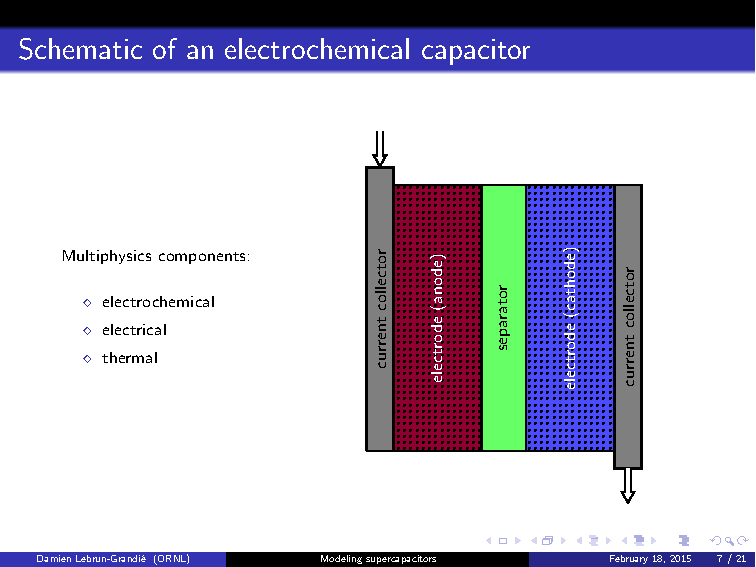
\includegraphics[trim = 2.4in 0.42in 0.7in 0.9in, clip, width=0.4\textwidth]{figures/supercap_schematic.pdf}  
    \caption{Schematic diagram of supercapacitors.}
    \label{fig:supercap}
\end{figure}

The current density in the matrix and solution phases can be expressed by Ohm's law as
%
\begin{eqnarray}
\mathbf{i}_1 &=& -\sigma\nabla\phi_1\\
\mathbf{i}_2 &=& -\kappa\nabla\phi_2
\end{eqnarray}
%
where $\mathbf{i}_1$ is the current density in solid matrix phase due to migration of electrons,
$\mathbf{i}_2$ is the  current density in the liquid electrolyte phase due to ion migration (assuming no concentration gradient and no convection due to bulk fluid motion),
$\phi_s$ and $\phi_2$ are potentials, and 
$\sigma$ is solid matrix electronic conductivity and $\kappa$ is liquid ionic conductivity.

Conservation of charge dictates that
\begin{equation}
I = \mathbf{i}_1 + \mathbf{i}_2
\end{equation}
and
\begin{equation}
-\nabla \cdot \mathbf{i}_1 = \nabla\cdot \mathbf{i}_2 = a {i}_n
\end{equation}

where $I$ is the total current density,
$a$ is the interfacial area per unit volume and the current transferred from the matrix phase to the electrolyte is the sum of the double-layer and the faradaic currents
\begin{equation}
{i}_n = C \frac{\partial}{\partial t} (\phi_1 - \phi_2)+
{i}_0 \left( \exp (\frac{\alpha_aF}{RT}\eta) - \exp (-\frac{\alpha_aF}{RT}\eta)
\right)
\end{equation}

where $C$ is the double-layer capacitance, ${i}_0$ is the exchange current density, $\alpha_{a}$ and $\alpha_{a}$ the anodic and cathodic charge transfer coefficients, respectively. $F$, $R$, and $T$ stand for Faraday’s constant, the universal gas constant and temperature. In the above relation, $\eta$ is the overpotential, defined as the difference between solid and liquid potentials with the equilibrium potential $U_{eq}$ as reference,
\[
\eta = \Delta \phi - U_{eq} = \phi_1 - \phi_2 - U_{eq}.
\]

For the simplest scenario of an ideally polarizable electrode, i.e. no Faradaic processes, a current transferred from the solid matrix to the solution phase goes towards only charging the double-layer at the electrode/electrolyte interface. This implies that:
%
\begin{equation}
\nabla\cdot \mathbf{i}_2 = \frac{\partial a q}{\partial t} = aC\frac{\partial \eta}{\partial t}
\end{equation}
%
where $q$ is the surface charge density of the double layer such as
%
\begin{equation}
q = C\Delta\phi = C(\phi_1 - \phi_2) = C\eta
\end{equation}
%

\subsection{Governing equation}
Assuming:
\begin{enumerate}[i.]

\item The electrical resistivity of the current collector is low (or it is sufficiently thin) that one can assume uniform distribution of $\phi_1$ over the collector domain: \textit{homogeneous in the $x$-direction}, 

\item There is no electron/ion fluxes cross the top and bottom boundaries (zero Neumann). Also due to high conductivity of collectors, the voltage over the whole interface on the collector side is negligible (similar to case that tab on the left collector is grounded): \textit{2D domain could be reduced to a quasi-1D domain},

\item The material properties are constant within a layer,

\end{enumerate}
%
the governing equations of the supercapacitor system reduce to
%
\begin{eqnarray}
aC\frac{\partial\eta}{\partial t} &=& -\kappa\frac{\partial^2\phi_2}{\partial x^2} \\ 
aC\frac{\partial\eta}{\partial t} &=& -\sigma\frac{\partial^2\phi_1}{\partial x^2} \label{eq:eta_phi1}\\ 
\kappa\frac{\partial^2\phi_2}{\partial x^2} &=& 0 
\end{eqnarray}
%
where the first two relations hold in the interior of the porous electrodes and the last one holds in interior of the separator ($\mathbf{i}_1=0$).

\textit{Boundary conditions:}
Assuming that a constant current is applied at one of the current collectors during charging/discharging, while the other current collector is grounded (Figure \ref{fig:schematic}), the boundary condition for a domain with electrode width of $L$ and separator width of $s$ can be written as
%
\begin{equation}
\left\{\begin{matrix}
\mathbf{i}_2 = 0; \mathbf{i}_1=-I & ;& x=0\\ 
\mathbf{i}_1 = 0  & ;& x=L\\ 
\mathbf{i}_1 = 0   & ;& x=L+s\\ 
\mathbf{i}_2 = 0 ; \phi_1=0 & ;& x=2L+s\\ 
-\kappa\frac{\partial\phi_2}{\partial x}|_{x=L} = -\kappa\frac{\partial\phi_2}{\partial x}|_{x=L+s} & &
\end{matrix}\right.
\end{equation}
%
where $I$ is the total current density at the current collector during charging or discharging.

\textit{Initial conditions:} 
%
\begin{equation}
\phi_1(x;t=0)  = \phi_1^0; \phi_2(x;t=0) = \phi_2^0;
\end{equation}
%
where $\phi_1^0=\phi_2^0$ for the case that the supercapacitor is initially fully discharged.

\begin{figure}[h]
    \centering
    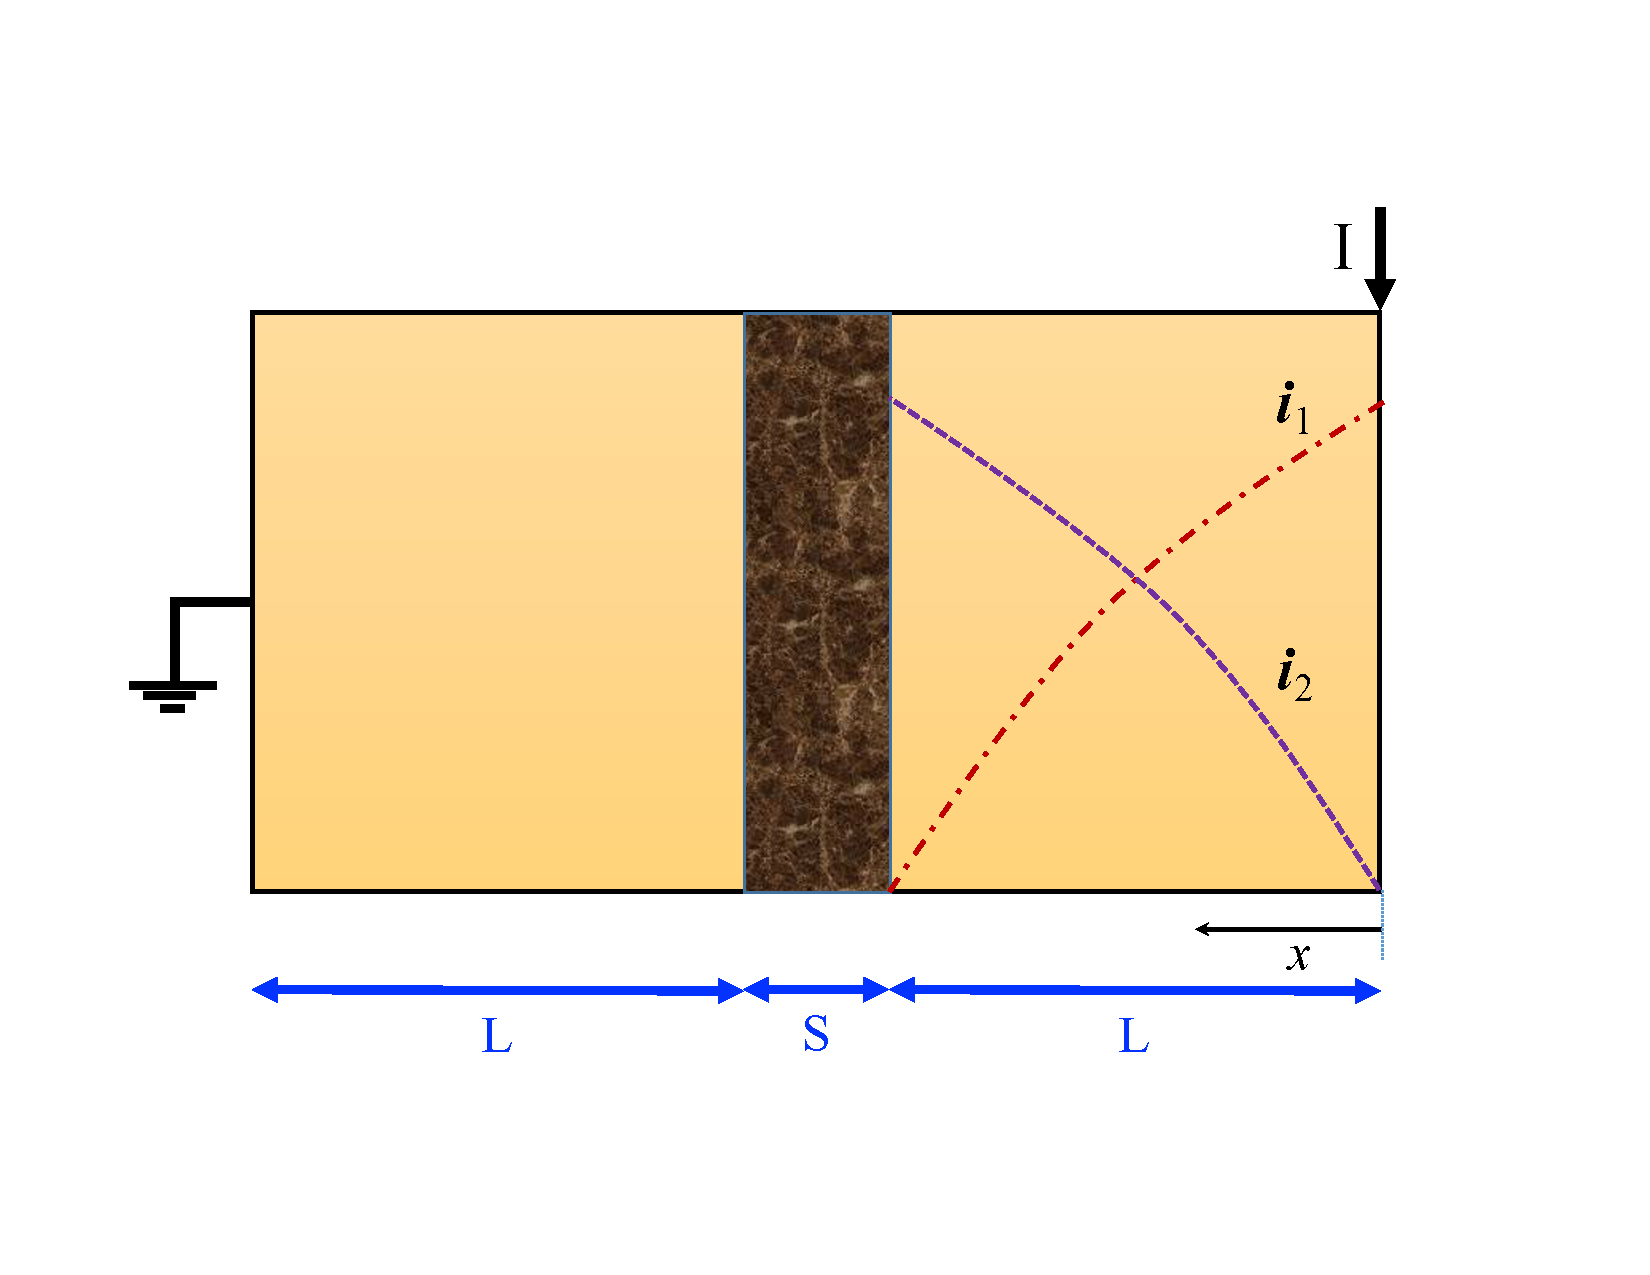
\includegraphics[trim = 0in 1.4in 0in 1.4in, clip, width=0.8\textwidth]{figures/schematic.pdf}  
    \caption{Schematic diagram of the supercapacitor considered here.}
    \label{fig:schematic}
\end{figure}


One can consider the cell voltage as a QoI in supercapcitors, which is defined as the potential drop across the system, $V_{cell} = \Delta\phi_{cell} = \phi_{collector}^L-\phi_{collector}^R$.
The voltage of a cell consisting of two (identical) electrodes with a separator between them can be evaluated using  
%
\begin{equation}\label{eq:cellvoltage}
V_{cell} = 2V_0 - 2V_{electrode} - V_{seperator}
\end{equation}
%
where $V_0$ accounts for the initial voltage of the cell, 
and $V_{seperator}$ and $V_{electrode}$ accounts for the potential drop across seperator and each of the electrodes respectively and they can be written as
%
\begin{eqnarray}
V_{seperator} &=&  I\frac{S}{\kappa_s} \\
V_{electrode} &=& \phi_1|_{x =0} - \phi_2|_{x =L}
\end{eqnarray}



%========================================================================
\section{Overpotential Through Electrodes}
%========================================================================

Following dimensionless variables are taken into account, 
%
\begin{eqnarray}
\xi &=& \frac{x}{L}\\
\gamma &=& \frac{\kappa}{\sigma}\\
\tau &=& \frac{\kappa\sigma}{\kappa+\sigma}\frac{t}{aCL^2}\\
\beta &=& \frac{S}{\kappa_s}\frac{\kappa\sigma}{L(\kappa+\sigma)}\\
I^* &=& I \frac{L}{V_0}\frac{\kappa+\sigma}{\kappa\sigma} \label{eq:Iscale}
\end{eqnarray}
%


%========================================================================
\subsection{High Fidelity model}

The non-dimensional governing equation for the 1D model can be written as follow: 
%
\begin{equation}\label{eq:HF}
\boxed{
{\rm High \; Fidelity \; model: \quad}
\frac{\partial\eta_{HF}}{\partial\tau} = \frac{\partial^2\eta_{HF}}{\partial\xi^2}
}
\end{equation}
%
Since the current is equal to the matrix phase and solution phase current at $x=0$ and $x=L$, respectively, the following BCs hold for the PDE (\ref{eq:HF})
%
\begin{eqnarray}\label{eq:HF_bcs}
\xi = 0 &\rightarrow& \frac{\partial\eta_{HF}}{\partial\xi}=-I^*\frac{\gamma}{1+\gamma}\\
\xi = 1 &\rightarrow& \frac{\partial\eta_{HF}}{\partial\xi}= I^*\frac{1}{1+\gamma} \nonumber
\end{eqnarray}
%
One can assume the general IC as 
%
\begin{equation}
\eta(\xi,\tau=0) = \eta_0(\xi)
\end{equation}
%

Having the BCs and IC,
one can write the exact solutions of the PDE (\ref{eq:HF}) for $\eta_0(\xi)=0$ as 

\begin{eqnarray}\label{eq:exactHF}
\eta_{HF} &=& I^*\tau + \frac{I^*(3\xi^2-1)}{6(1+\gamma)} + \frac{I^*\gamma(3\xi^2+2-6\xi)}{6(1+\gamma)}\\
	 &-& \frac{2I^*}{\pi^2(1+\gamma)} \sum_{n=1}^\infty \left[\frac{(-1)^n+\gamma}{n^2} \right] \cos(n\pi\xi) \exp(-n^2\pi^2\tau). \nonumber
\end{eqnarray}




%========================================================================
\subsection{Low Fidelity model}


The upscaled (averaged) model can be developed simply by spatially
average the governing equation over the entire domain length in the $x$-direction. Therefore PDE of the HF model reduces to an ODE 
%
\begin{equation}\label{eq:LF_avg}
\frac{\partial{\eta}_{LF}^{avg}}{\partial\tau} = I^*
\end{equation}

One can assume a quadratically varying profile for overpotential inside the electrodes \cite{subramanian2001}
\begin{equation}\label{eq:quadratic}
\eta_{LF} (\xi,\tau)= a(\tau)\xi^2 + b(\tau)\xi + c(\tau)
\end{equation}

Using BCs in (\ref{eq:HF_bcs}) one can obtain
\begin{equation}\label{eq:a_b}
a(\tau) = \frac{1}{2}I^* \qquad;\qquad b(\tau) = -I^*\frac{\gamma}{1+\gamma}
\end{equation}

An spatial averaged overpotential can be determined using (\ref{eq:quadratic}):
\begin{equation}
\eta_{LF}^{avg} (\tau) = \int_0^1 \eta_{LF} \; d\xi = \frac{a(\tau)}{3} + \frac{b(\tau)}{2} + c(\tau)
\end{equation}

Computing $c(\tau)$ from above equation, one can re-write (\ref{eq:quadratic}) as 
%
\begin{equation}\label{eq:LF}
\boxed{
{\rm Low\; Fidelity \; model: \quad}
\eta_{LF}(\xi,\tau) = 
\frac{1}{2}I^*(\tau)\xi^2 - I^*(\tau) \frac{\gamma}{1+\gamma}\xi + {\eta}_{LF}^{avg}(\tau) - \frac{I^*(\tau)}{6} + \frac{I^*(\tau)}{2}\frac{\gamma}{1+\gamma}
}
\end{equation}
%
where ${\eta}_{LF}^{avg}(\tau)$ is the solution of (\ref{eq:LF_avg}) given appropriate initial condition.




%========================================================================
\section{Cell Voltage}
%========================================================================

The QoI, cell voltage (\ref{eq:cellvoltage}), needs to be computed from the overpotential values. The potential drop across the electrode can be derived by substituting of the dimensionless variables in (\ref{eq:eta_phi1}) 
%
\begin{equation}\label{eq:eta_phi_nondim_pde}
\frac{\partial^2\phi_1}{\partial\xi^2} = \frac{-\gamma}{1+\gamma}\frac{\partial\eta}{\partial\tau} = \frac{-\gamma}{1+\gamma}\frac{\partial^2\eta}{\partial\xi^2}
\end{equation}
%
along with the boundary conditions for $\phi_1$ and $\eta$
%
\begin{eqnarray}
\xi = 0 &\rightarrow& \frac{\partial\eta}{\partial\xi}= -I^*\frac{\gamma}{1+\gamma} \\
\xi = 1 &\rightarrow& \frac{\partial\eta}{\partial\xi}= I^*\frac{1}{1+\gamma}
\end{eqnarray}

\begin{eqnarray}
x = 0   : \mathbf{i}_1=-\sigma	\frac{\partial\phi_1}{\partial x}= -I  \; &\rightarrow& \;   
\xi = 0 : \frac{\partial\phi_1}{\partial\xi}= \frac{LI}{\sigma} \\
x = L   : \mathbf{i}_1=-\sigma	\frac{\partial\phi_1}{\partial x}= 0  \;  &\rightarrow& \; 
\xi = 1 : \frac{\partial\phi_1}{\partial\xi}= 0 \label{eq:phi1_bc}
\end{eqnarray}

Integrating (\ref{eq:eta_phi_nondim_pde}) with respect to $\xi$ yields
%
\begin{equation}
\frac{\partial\phi_1}{\partial\xi} = \frac{-\gamma}{1+\gamma}\frac{\partial\eta}{\partial\xi} + A
\end{equation}
%
and using (\ref{eq:phi1_bc}) to determine $A$, results in following relation
%
\begin{equation} \label{eq:eta_phi_nondim_pde1}
\frac{\partial\phi_1}{\partial\xi} = \frac{-\gamma}{1+\gamma}\frac{\partial\eta}{\partial\xi} + I^*\frac{\gamma}{(1+\gamma)^2}
\end{equation}
%
Integrating (\ref{eq:eta_phi_nondim_pde1}) between the limits $\xi=0$ to $1$ gives the charge in the dimensionless solid phase potential across the electrode
%
\begin{equation} \label{eq:eta_phi_ends}
\phi_1|_{\xi=1} - \phi_1|_{\xi=0} = 
\frac{-\gamma}{1+\gamma}\left(\eta|_{\xi=1} - \eta|_{\xi=0}\right) + I^*\frac{\gamma}{(1+\gamma)^2}
\end{equation}
%

Using (\ref{eq:eta_phi_ends}), the dimensionless potential drop across the porous electrode can be written as
%
\begin{eqnarray}\label{eq:Vellectrod}
V^*_{electrode} &=& \phi_1|_{\xi=0} - \phi_2|_{\xi=1} = \eta|_{\xi=1} + (\phi_1|_{\xi=0} - \phi_1|_{\xi=1})\\
				&=&  \frac{1+2\gamma}{1+\gamma}\eta|_{\xi=1} - \frac{\gamma}{1+\gamma}\eta|_{\xi=0} - I^*\frac{\gamma}{(1+\gamma)^2}
\end{eqnarray}
%

Having the exact values of overpotentials at the boundaries from HF model (\ref{eq:exactHF}) and LF model (\ref{eq:LF}) one can obtained the potential across the electrode 
%
\begin{eqnarray}\label{eq:Velec_HF_LF}
V^*_{electrode-HF} &=&  I^* \left( \frac{1}{3} +\tau - 2 \sum_{n=1}^\infty \frac{1}{n^2\pi^2}\left(\frac{(-1)^n\gamma}{1+\gamma} + \frac{1}{1+\gamma} \right)^2 \exp (-n^2\pi^2\tau)  \right)\\
V^*_{electrode-LF} &=&   \eta_{LF}^{avg} + I^*\left(  \frac{2\gamma+1}{3\gamma+1} + \frac{5}{3}\frac{\gamma}{1+\gamma} - \frac{\gamma}{1+\gamma^2} \right)
\end{eqnarray}
%%

Substituting the above relation into (\ref{eq:cellvoltage}) one can compute the cell voltage as QoI: $Q = V_{cell}$ as
%
\begin{equation}\label{eq:Vcell}
V_{cell}^* = \frac{V_{cell}}{2V_0} = 1 - \frac{1}{2}\beta I^* - V^*_{electrode}
\end{equation}
%

%========================================================================
\section{Model Inadequacy Formulation}
%========================================================================

%========================================================================
\subsection{Summary of a posterior estimation of modeling error}
We consider an abstract variational problem of finding an element $u$ in a topological vector space $\mathcal{V}$ such that,
%
\begin{equation}\label{B_F2}
\mathcal{B} (u ; v) = \mathcal{F}(v), \qquad \forall v \in \mathcal{V},
\end{equation}
%
%
where $\mathcal{B(\cdot ; \cdot)}$ is a semilinear form from $\mathcal{V} \times \mathcal{V}$ into $\mathbb{R}$ and $\mathcal{F}$ is a linear functional on $\mathcal{V}$. Problem (\ref{B_F2}) is equivalent to the problem of finding a solution $u$ of the problem $A(u)=F$ in the dual space $\mathcal{V}'$, where $A$ is the map induced by $\mathcal{B(\cdot ; \cdot)} : \langle A(u),v \rangle = \mathcal{B} (u ; v) = \mathcal{F}(v) = \langle \mathcal{F}, v \rangle$, $\langle \cdot ; \cdot\rangle$ denoting duality pairing in $\mathcal{V}' \times \mathcal{V}$.
Assuming (\ref{B_F2}) is solvable for $u$, we wish to compute the value $Q(u)$ of a functional $Q: \mathcal{V} \rightarrow \mathbb{R}$ representing a quantity of interest, or an observable of interest.

We assume that the semilinear form $\mathcal{B} ( \cdot ; \cdot )$ and the functional $Q ( \cdot ; \cdot )$ are three times Gateaux differentiable on $\mathcal{V}$ with respect to $u$. In particular, the following limits exist,
%
\begin{equation}
\left.\begin{matrix}
\mathcal{B}'(u; w, v) & = & \lim_{\theta \rightarrow 0} & \theta^{-1} \left[ \mathcal{B}(u+\theta w, v) - \mathcal{B}(u, v) \right] \\ 
Q' (u;v) & = & \lim_{\theta \rightarrow 0} & \theta^{-1} \left[ Q(u+\theta v) - Q(u) \right ]
\end{matrix}\right\}.
\end{equation}
%
%
with similar definitions of higher-order derivatives, e.g. $\mathcal{B}''(u; w_1, w_2,v)$, $\mathcal{B}'''(u; w_1,\\ w_2, w_3, v)$, $Q''(u; w, v)$, $Q''(u; v_1, v_2, v_3)$, etc. 

The adjoint problem associated with (\ref{B_F2}) and the quantity of interest $Q$ consists of finding $z \in \mathcal{V}$ such that 
%
\begin{equation}\label{Bprime_Qprime2}
\mathcal{B}' (u; z, v) = Q' (u; v), \qquad \forall v \in \mathcal{V}.
\end{equation} 



Now let $u_0$ be an arbitrary element selected in $\mathcal{V}$. The residual functional (or ``residuum'') associated with $u_0$ is defined as the semilinear functional $\mathcal{R}: \mathcal{V} \times \mathcal{V} \rightarrow \mathbb{R}$,
%
\begin{equation}
\mathcal{R} (u_0; v) = \mathcal{F}(v) - \mathcal{B}(u_0;v),
\end{equation}
%
%
which, for each $u_0 \in \mathcal{V}$, is a linear functional on $\mathcal{V}$.

Obviously, if $u_0 = u$, the solution of (\ref{B_F2}), $\mathcal{R}(u;v)=0 \;\; \forall v \in \mathcal{V}$.
Thus, $\mathcal{R}(u_0;v)$ describes the degree to which the vector $u_0$ fails to satisfy the central problem (\ref{B_F2}).

We now recall the basic theorem in \cite{oden2006}:
%
\begin{theorem}\label{theorem:1} 
Let the semilinear form $\mathcal{B}(\cdot ; \cdot)$ in (\ref{B_F2}) and the quantity of interest $Q$ be three-times continuously Gateaux differentiable on $\mathcal{V}$.
Let $u_0$ be an arbitrary element of $\mathcal{V}$.
Then the error in $Q(u)$ produced by replacing $u$ by $u_0$ is given by:
%
\begin{equation}\label{Qu_Qu0}
Q(u) - Q(u_0) = \mathcal{R}(u_0;z) + \Delta
\end{equation}
%
where $\Delta$ is a remainder involving higher-order terms in $e_0 = u - u_0$ and $\varepsilon_0 = z - z_0$, $z_0$ being an approximation of $z$.
\end{theorem}An explicit form of $\Delta$ is given in the appendix.


If $u_0$ is not an arbitrary vector taken from $\mathcal{V}$ but is a solution of a surrogate problem approximating ($\ref{B_F2}$)
(such as a coarse-grained model approximating an AA model), then it often happens that $\Delta$ is negligible compared to the residual. Then (\ref{Qu_Qu0}) reduces to the approximation,
%
\begin{equation}\label{Qu_Qu0_noreminder}
Q(u) - Q(u_0) \approx \mathcal{R}(u_0;z).
\end{equation}
 
This relation is the basis for many successful methods of \textit{a posteriori} error estimation of both modeling error and numerical error. Whenever $\mathcal{B}(\cdot;\cdot)$ is a bilinear form and $Q(\cdot)$ is linear, $\Delta \equiv 0$.

%========================================================================
\subsection{Estimation of error in LF model }
Local residual can be obtained by substituting the solution of surrogate (LF) model into the base (HF) model such as
%
\begin{equation}
\rho(\xi, \tau) = \frac{\partial{\eta_{LF}}}{\partial\tau} - \frac{\partial^2{\eta_{LF}}}{\partial\xi^2},
\end{equation}
%
and with some manipulation one can obtain
%
\begin{equation}\label{eq:residual}
\rho(\xi, \tau) = \frac{\partial I^*}{\partial\tau} \left(
\frac{\xi^2}{2} - \frac{\gamma}{1+\gamma}\xi - \frac{1}{6} + \frac{\gamma}{2(1+\gamma)}
\right)
\end{equation}


Moreover, error in overpotential produced by using the surrogate model is defined as
%
\begin{equation}\label{eq:error}
\epsilon(\xi,\tau) = \eta_{HF} - \eta_{LF}
\end{equation}
%
Accordingly, the evolution of the error in space and time could be expressed as
%
\begin{equation}\label{eq:errorPDE}
\frac{\partial\epsilon}{\partial\tau} = \frac{\partial^2\epsilon}{\partial\xi^2} - \rho(\xi,\tau)
\end{equation}
%

Having, 
%
\begin{equation}
\frac{\partial\epsilon}{\partial\xi} = \frac{\partial(\eta_{HF}-\eta_{LF})}{\partial\xi}
 = \frac{\partial\eta_{HF}}{\partial\xi}-(I^*\xi-I^*\frac{\gamma}{1+\gamma})
\end{equation}
%
along with (\ref{eq:HF_bcs}), the boundary conditions of PDE (\ref{eq:errorPDE}) can be written as,
\begin{eqnarray}\label{eq:error_bcs}
\xi = 0 &\rightarrow& \frac{\partial\epsilon}{\partial\xi}= 0\\
\xi = 1 &\rightarrow& \frac{\partial\epsilon}{\partial\xi}= 0. \nonumber
\end{eqnarray}

Initial condition of (\ref{eq:errorPDE}) can be easily obtained as
\begin{equation}
\epsilon(\xi,\tau=0) = \eta_{HF}(\xi,\tau=0) - {\eta}_{LF}(\xi,\tau=0) = \epsilon_0(\xi)
\end{equation}

Having the BCs and IC,
one can write the exact solutions of the PDE (\ref{eq:errorPDE}) using separation of variables as

\begin{equation}
\epsilon(\xi,\tau) = \sum_{n=1}^{\infty} \phi_n \exp(-(n\pi)^2\tau) \cos(n\pi\xi) - A_n \cos(n\pi\xi) \int_0^{\tau} \exp\left(-(n\pi)^2(\tau - S) \right) \frac{\partial I^*}{\partial\tau} dS
\end{equation}
\begin{eqnarray}
\phi_n &=& 2 \int_0^1 \epsilon_0(\xi) \cos(n\pi\xi) d\xi\\
A_n &=& \frac{1}{3(n\pi)^3(1+\gamma)}\left[
-6\gamma\sin(n\pi) - \sin(n\pi) + 2(n\pi)^2\sin(n\pi) + 6(n\pi)\gamma + 6(n\pi)\cos(n\pi) - \gamma(n\pi)^2\sin(n\pi)
\right]. \nonumber
\end{eqnarray}

For the special case of $\rho(\xi,\tau)=0$, e.g. constant current, the exact solution of (\ref{eq:errorPDE}) can be written as,
\begin{equation}
\epsilon(\xi,\tau) = A_0 + \sum_{n=1}^{\infty} A_n \exp\left(-(n\pi)^2\tau \right) \cos(n\pi\xi)
\end{equation}
\begin{eqnarray}
A_0 &=& \int_0^1 \epsilon_0(\xi) d\xi\\
A_n &=& \int_0^1 \epsilon_0(\xi) \cos(n\pi\xi) d\xi. \nonumber
\end{eqnarray}


Consequently, through the information about the evolution of the error and information from the local residual, it might be possible to formulate the error in QoI, cell voltage, incurred from solving the low-fidelity equation without having to solve the high-fidelity system of equations,
%
\begin{equation}
\mathcal{E} = Q(\eta_{HF}) - Q(\eta_{LF}) = V^*_{cell}(\eta_{HF}) - V^*_{cell}(\eta_{LF}).
\end{equation}


%========================================================================
\section{Numerical Example: Constant Current Discharge}
%========================================================================

In order to build intuition regarding the evolution of overpotential and cell voltage, we consider two simple numerical example with imposing constant and cyclic current, when the supercapcitor is initially fully discharged ($\phi_1(x;t=0) = \phi_2(x;t=0)=0$).
%
The values of the parameters considered in this example are presented in Table \ref{table:example}. 
%
%
\begin{table}[h]
\centering
\caption{Values of parameters for the illustrative example.}
\label{table:example}
\begin{tabular}{|l|l|}
\hline
$\kappa$ & 0.0195174 $sec/m$\\ \hline
$\sigma$ & 52.1  $sec/m$\\ \hline
$L$         & 50e-6  $m$\\ \hline
$C$         & 0.03134  $ F/m^2$\\ \hline
$a$         & 4.19956e7/C   $m$\\ \hline
$V_0$      & 1.25   $volt$\\ \hline
$I_{\rm unscaled}$ & 200  $Amp/m^2$\\ \hline
$\kappa_s$ & 0.0311627 $sec/m$\\ \hline
$S$         & 25e-6  $m$\\ \hline
\end{tabular}
\end{table}

%========================================================================
\subsection{Evolution of overpotential}

%================
\textit{Solution of LF model:}
Figures (\ref{fig:etaLF}) and (\ref{fig:etaLF_cycl}) show the variation of solution of LF model (\ref{eq:LF}) in the normalized time and space. $\eta_{LF}^{avg}$ in this equation is the solution of (\ref{eq:LF_avg}) such as
%
\begin{equation}\label{eq:Iprim}
{\eta_{LF}^{avg}}(\tau) = \int_0^{\tau} I^*(\tau') d\tau' 
 = I^* \tau
\end{equation}
%%
%%
\begin{figure}[h]
    \centering
    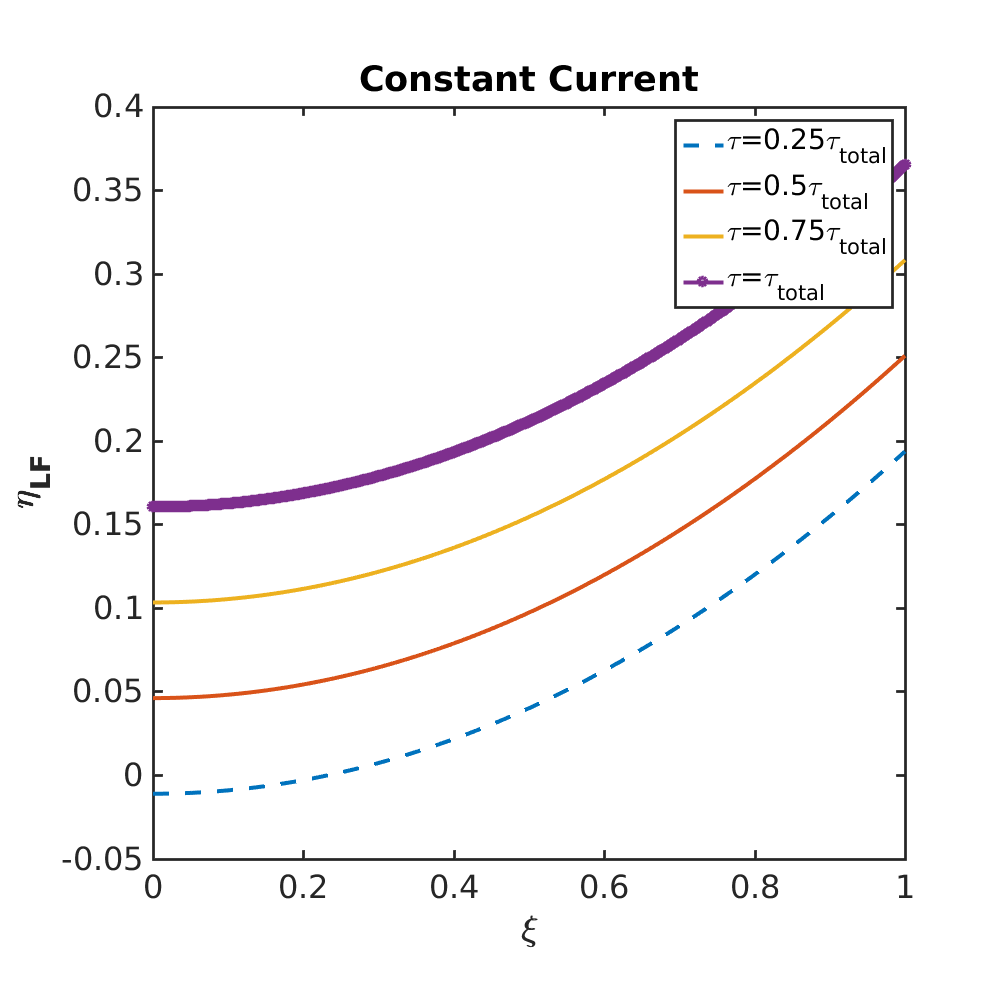
\includegraphics[trim = 0in 0in 0in 0in, clip, width=0.7\textwidth]{figures/etaLF2d.png}
    \\
    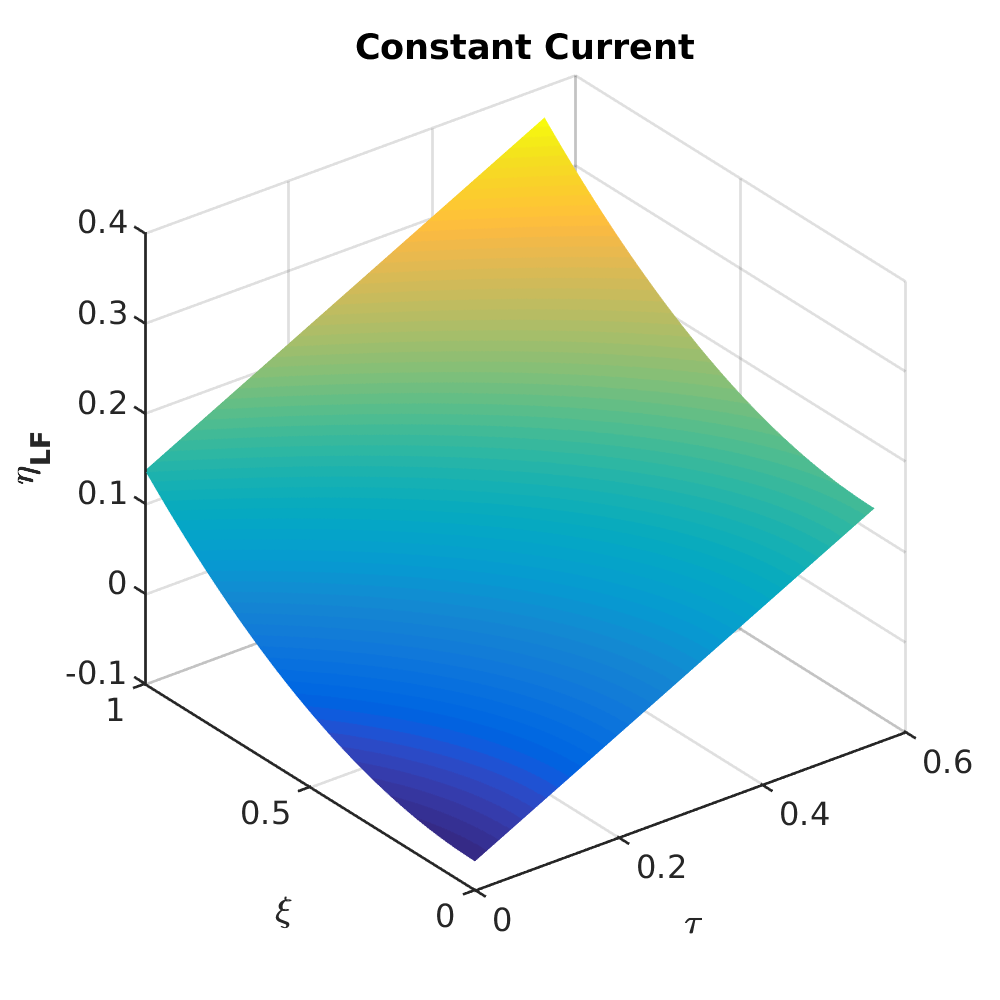
\includegraphics[trim = 0in 0in 0in 0in, clip, width=0.7\textwidth]{figures/etaLF3d.png}      
    \caption{Solution of LF model for constant current.}
    \label{fig:etaLF}
\end{figure}
%%
%
%================
\textit{Solution of HF model:}
Solution of the HF model is shown in Figures (\ref{fig:etaHF}) and (\ref{fig:etaHF_cycl}). The following PDE+BCs is solved using finite difference methods:

\begin{equation*}
\frac{\partial\eta}{\partial\tau} = \frac{\partial^2\eta}{\partial\xi^2}
\end{equation*}
%
\begin{eqnarray}
{\rm BCs:} & \frac{\partial\eta}{\partial\tau}|_{\xi=0} = -I^* \frac{\gamma}{1+\gamma} \;\; ; \;\;
\frac{\partial\eta}{\partial\tau}|_{\xi=1} = I^* \frac{1}{1+\gamma}\\
{\rm IC:} & \eta(\xi,\tau=0)=0
\end{eqnarray}
%
%%
\begin{figure}[h]
    \centering
    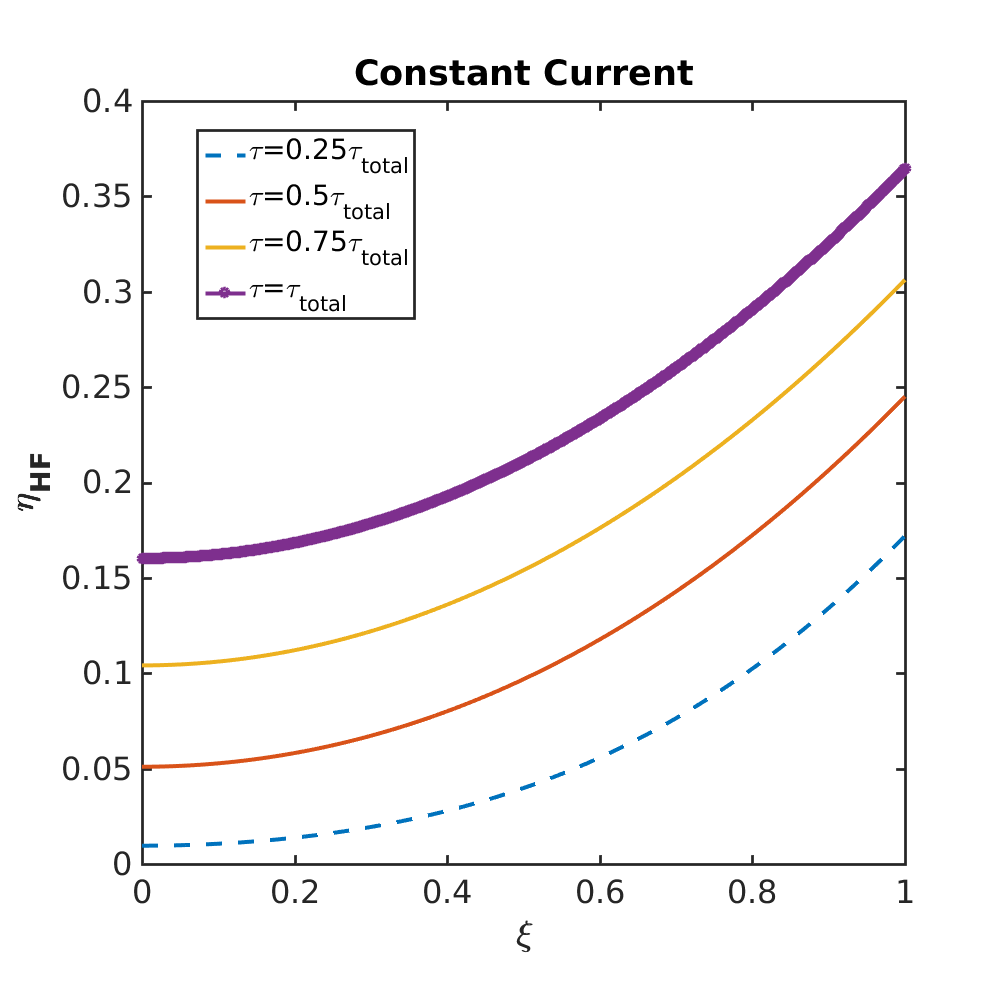
\includegraphics[trim = 0in 0in 0in 0in, clip, width=0.7\textwidth]{figures/etaHF2d.png}
    \\
    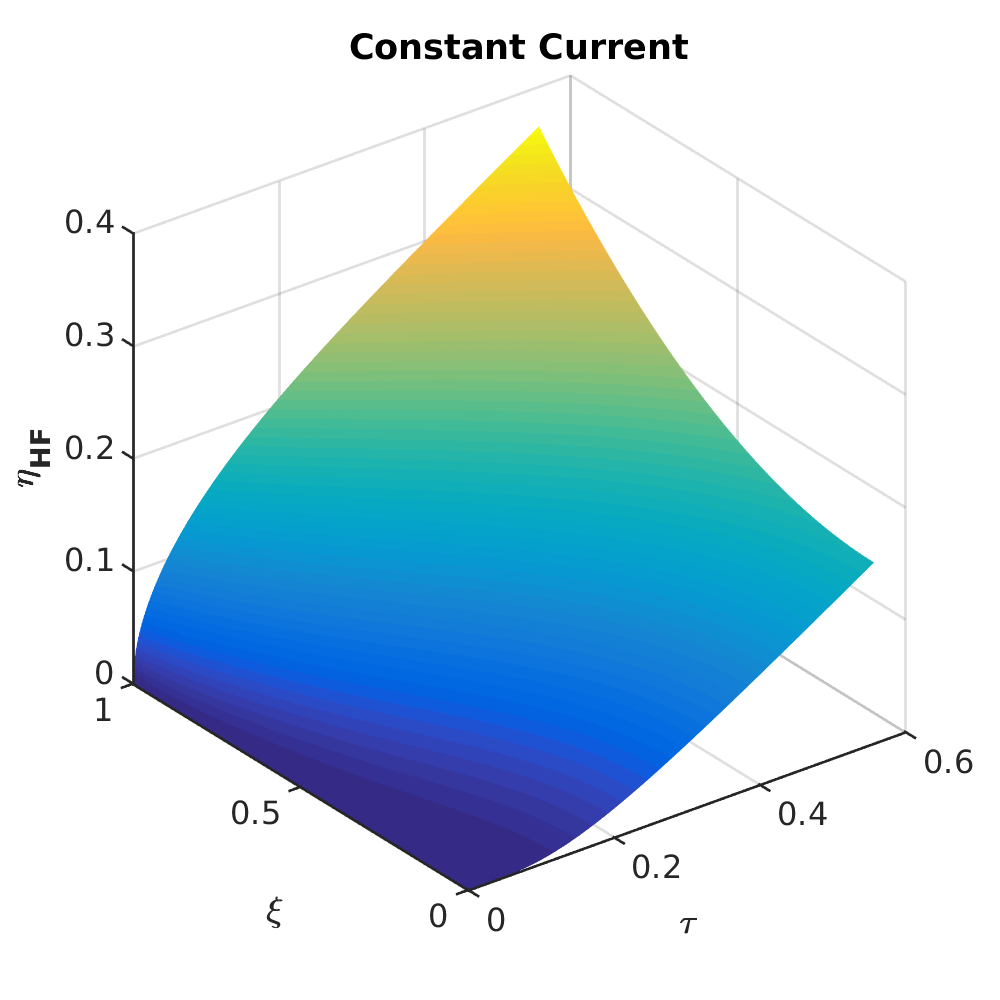
\includegraphics[trim = 0in 0in 0in 0in, clip, width=0.7\textwidth]{figures/etaHF3d.png}      
    \caption{Solution of HF model for constant current.}
    \label{fig:etaHF}
\end{figure}
%%


%============
\textit{Evolution of error:}
The local residual $\rho(\xi,\tau)$ can be computed from (\ref{eq:residual}). However, $\frac{\partial I}{\partial \tau} = 0 $ in both examples
resulting in zero local residual.


Having the solution of HF model one can obtain the exact error $\epsilon_{\rm exact} = \eta_{HF} - \eta_{LF}$. This can be compared with
the evolution of error that is obtained from solving the following PDE (Figures \ref{fig:error_2d} and \ref{fig:error_3d}).

\begin{equation*}
\frac{\partial\epsilon}{\partial\tau} = \frac{\partial^2\epsilon}{\partial\xi^2} -\rho(\xi,\eta)
\end{equation*}
%
\begin{eqnarray}
{\rm BCs:} & \frac{\partial\epsilon}{\partial\xi}|_{\xi=0} = \frac{\partial\epsilon}{\partial\xi}|_{\xi=1} = 0\\
{\rm IC:} & \epsilon(\xi,\tau=0) = \eta_{HF}(\xi,\tau=0) - \eta_{LF}(\xi,\tau=0)
\end{eqnarray}
%


%%
\begin{figure}[h]
    \centering
    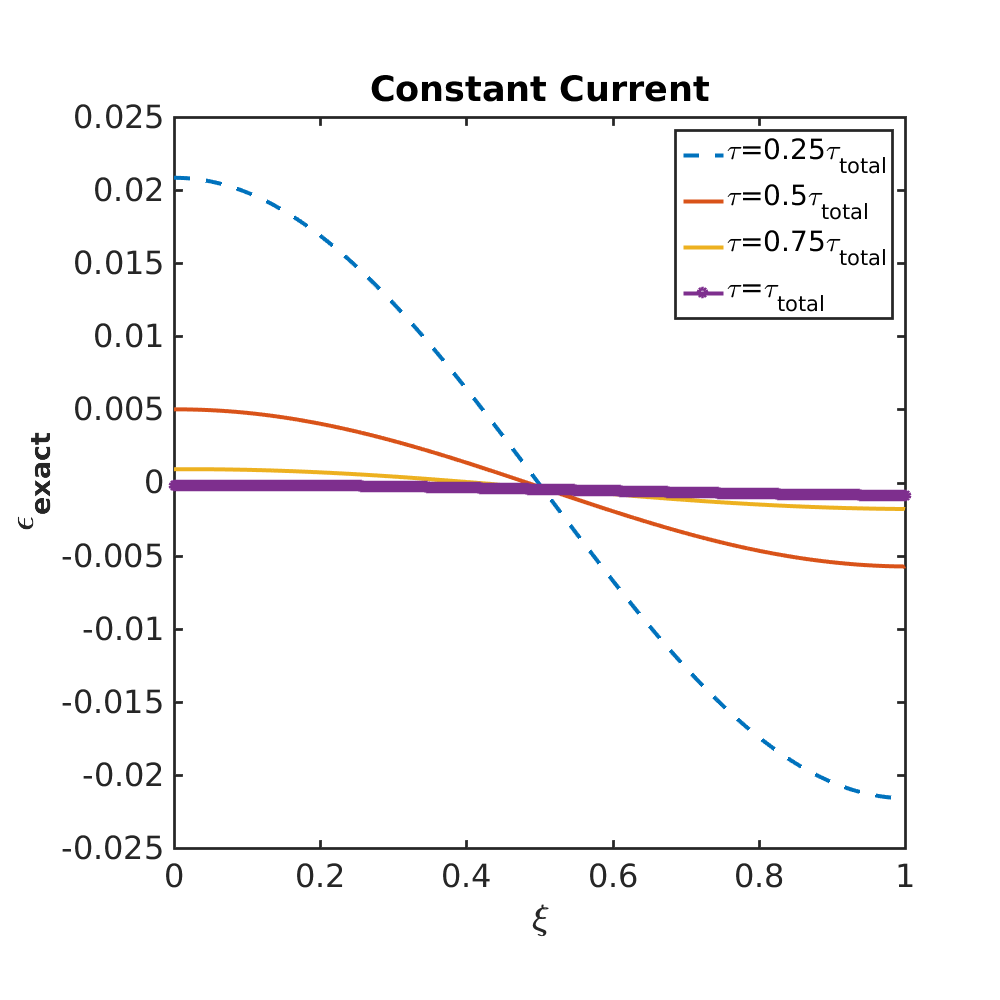
\includegraphics[trim = 0in 0in 0in 0in, clip, width=0.7\textwidth]{figures/error2d_exact.png}
    \\
    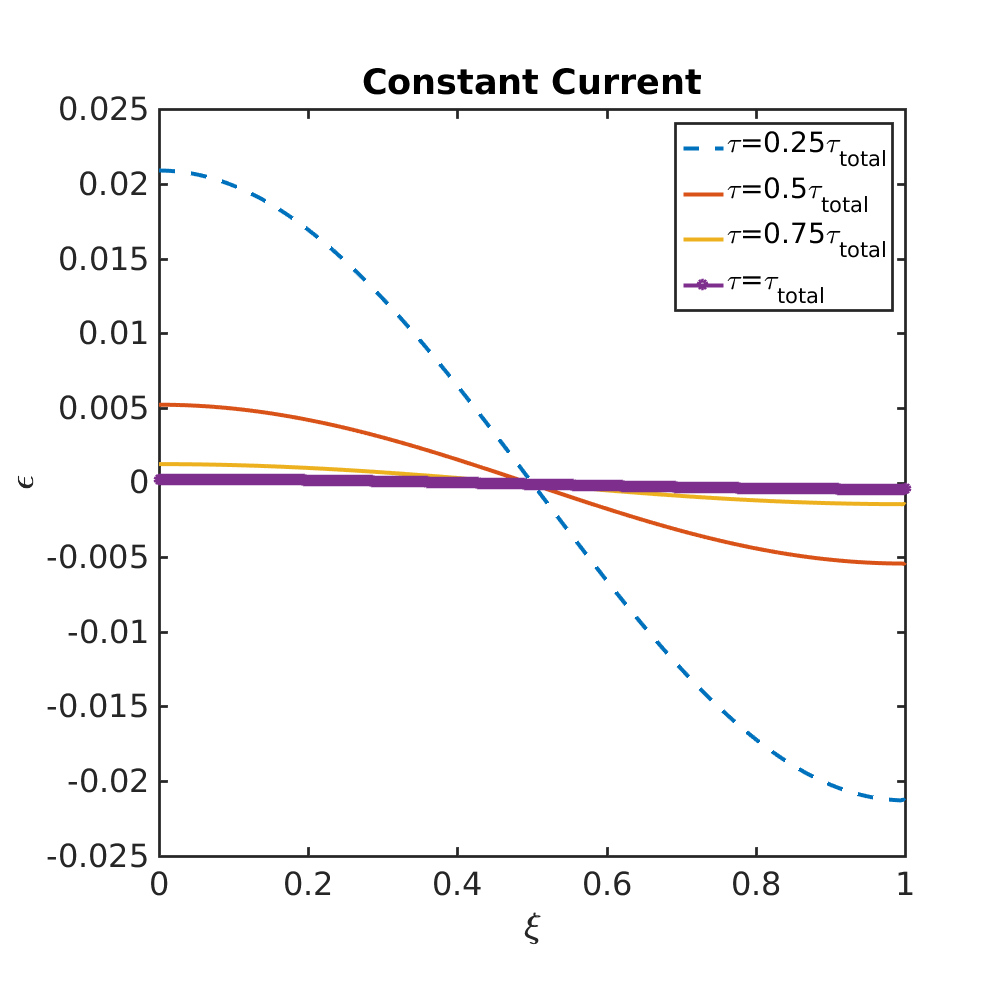
\includegraphics[trim = 0in 0in 0in 0in, clip, width=0.7\textwidth]{figures/error2d.png}      
    \caption{Solution of error $\epsilon(\xi,\tau)$ at different normalized time and space : (top) exact error using HF model, (bottom) error using (\ref{eq:error}).}
    \label{fig:error_2d}
\end{figure}
%%
%%
\begin{figure}[h]
    \centering
    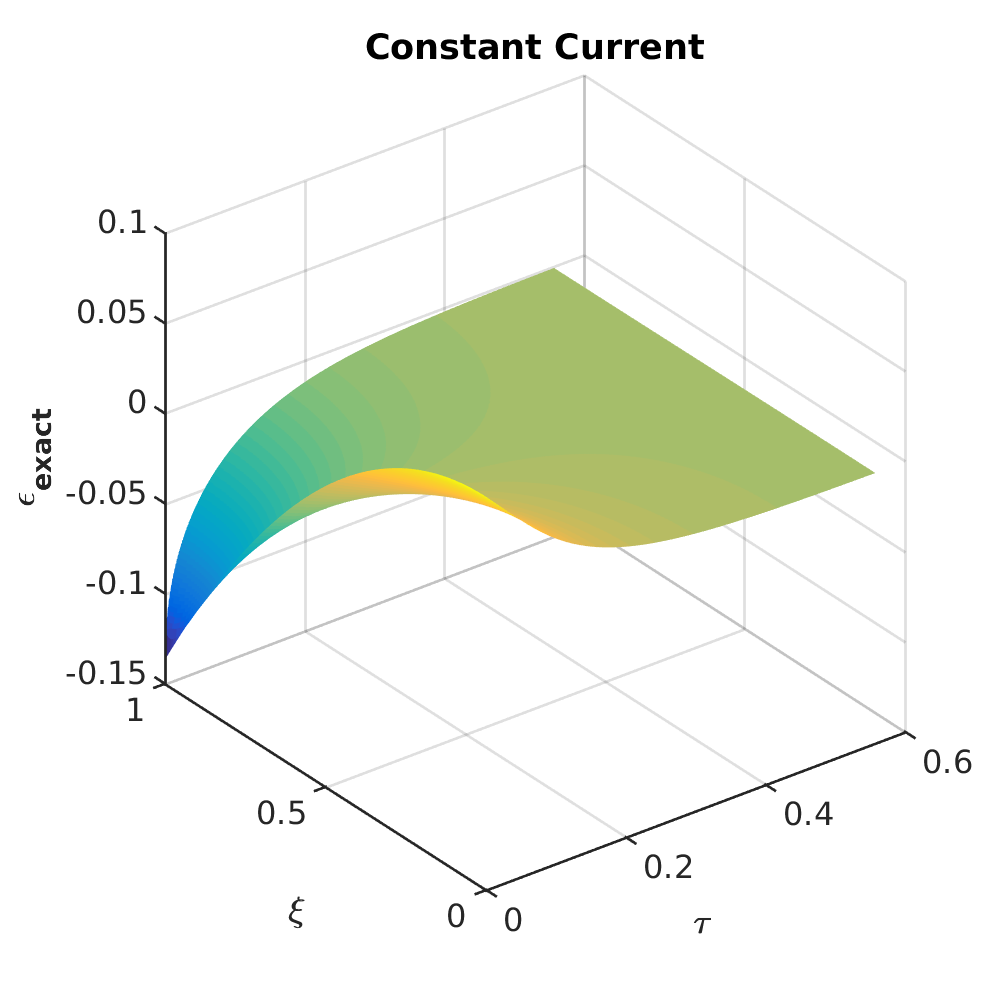
\includegraphics[trim = 0in 0in 0in 0in, clip, width=0.7\textwidth]{figures/error3d_exact.png}
    \\
    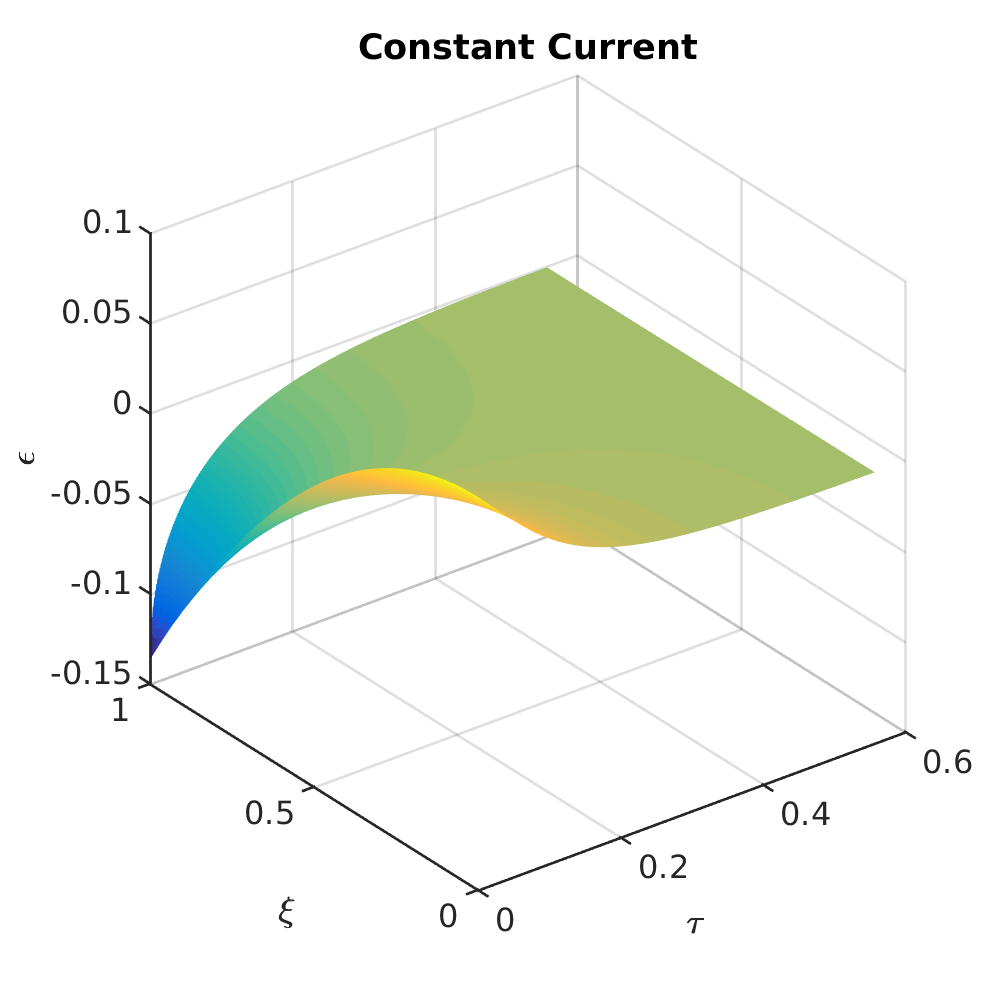
\includegraphics[trim = 0in 0in 0in 0in, clip, width=0.7\textwidth]{figures/error3d.png}      
    \caption{Solution of error $\epsilon(\xi,\tau)$ at different normalized time and space : (top) exact error using (\ref{eq:error}) and solution of HF model, (bottom) error using (\ref{eq:errorPDE}).}
    \label{fig:error_3d}
\end{figure}
%%



%========================================================================
\subsection{Time evolution of cell voltage}

Having the solutions of overpotential furnished by HF and LF model, the time evolution of the normalized voltage can be computed using (\ref{eq:Vcell}). The results are shown in Figures (\ref{fig:Vcell}) and (\ref{fig:Vcell_cycl}).

%%
\begin{figure}[h]
    \centering
    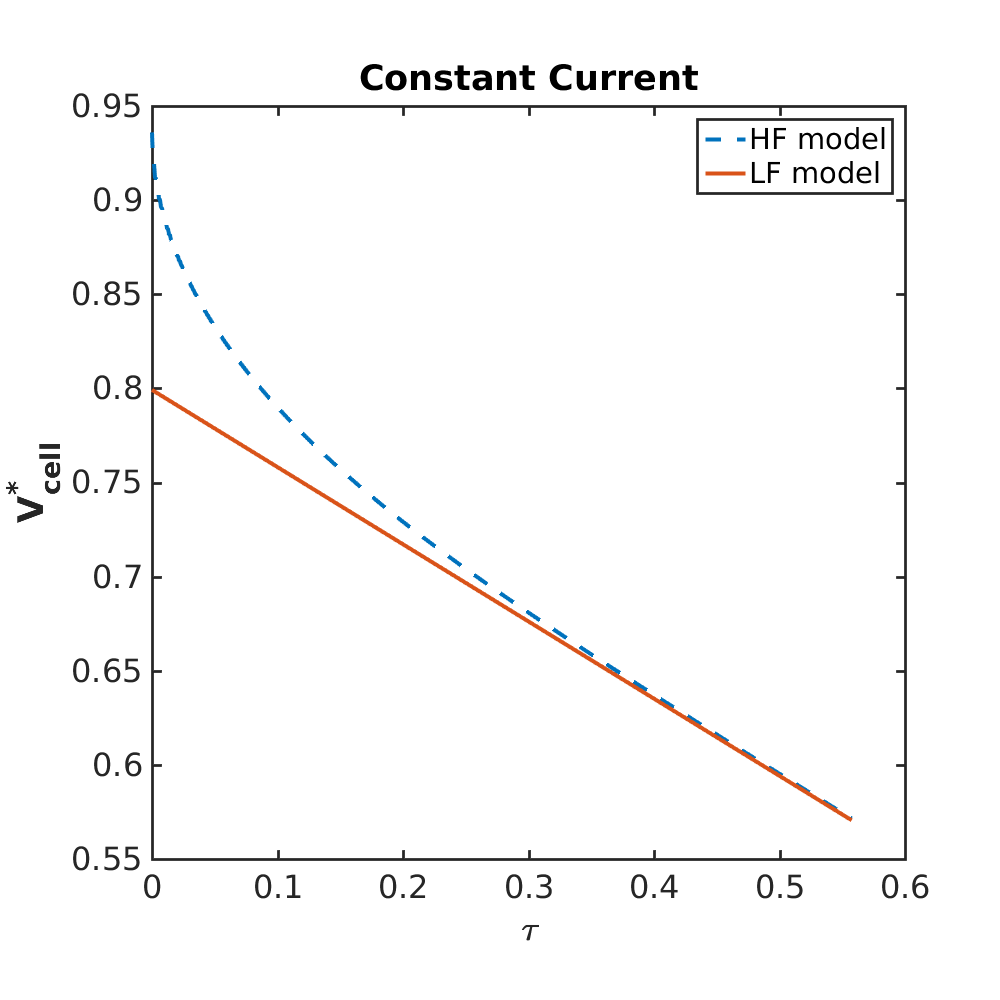
\includegraphics[trim = 0in 0in 0in 0in, clip, width=1.1\textwidth]{figures/Vcell.png}      
    \caption{Change in voltage across the porous electrode with dimensionless time for constant current.}
    \label{fig:Vcell}
\end{figure}
%%


%========================================================================
%		Results of Cyclic I
%========================================================================


%%
\begin{figure}[h]
    \centering
    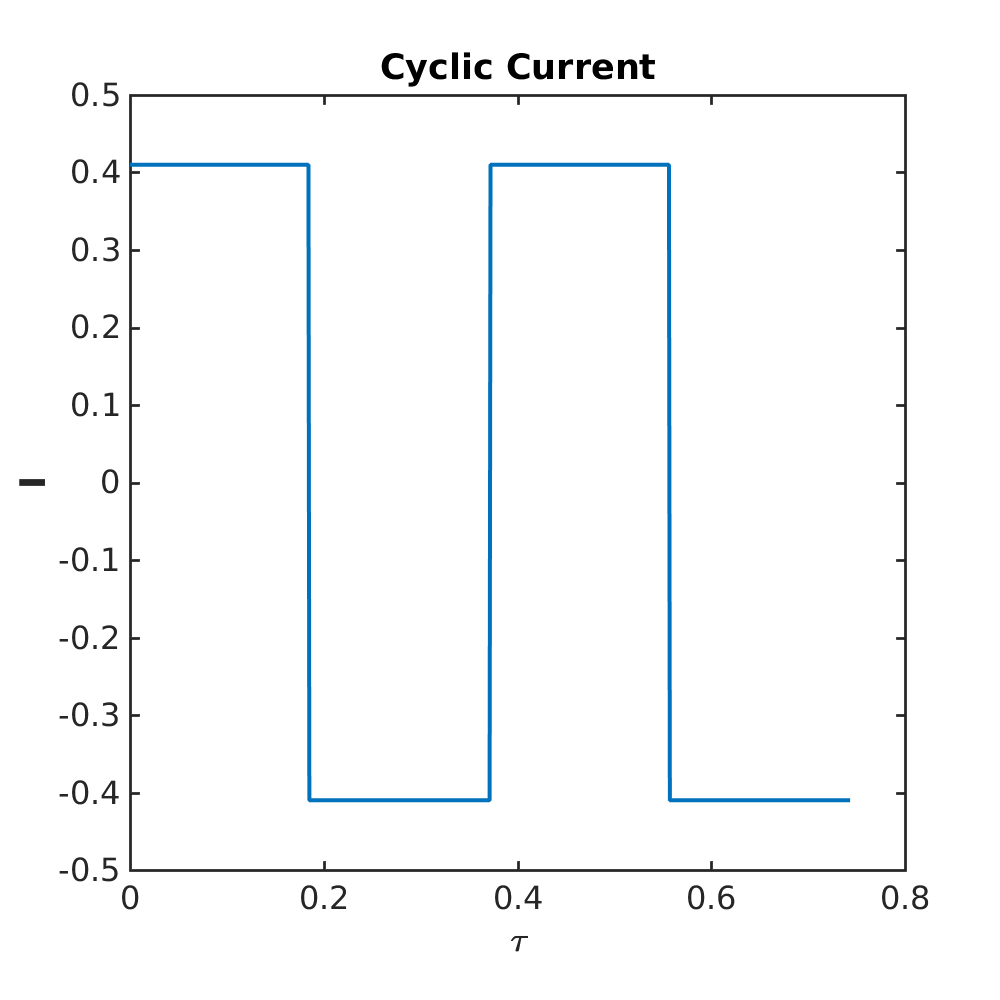
\includegraphics[trim = 0in 0in 0in 0in, clip, width=1.1\textwidth]{figures/I_cycl.png}      
    \caption{Cyclic current imposed.}
    \label{fig:I_cycl}
\end{figure}
%%


%%
\begin{figure}[h]
    \centering
    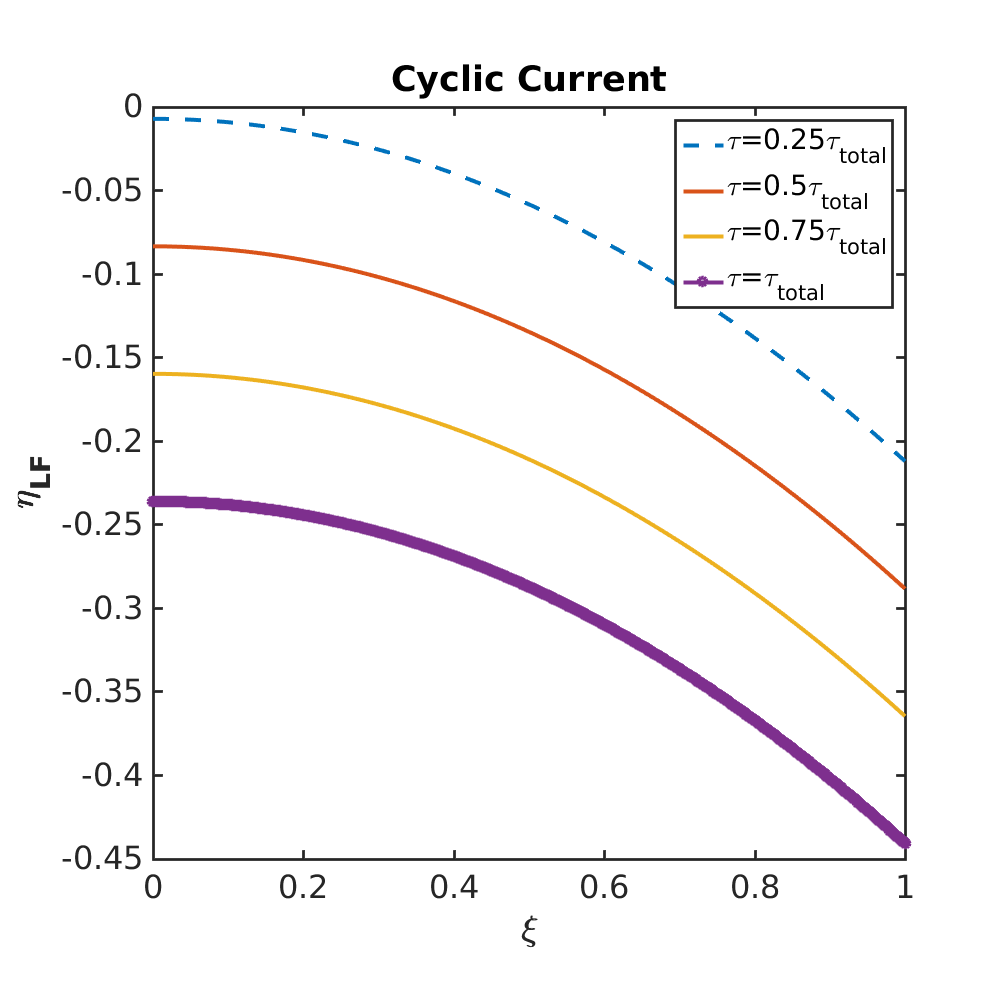
\includegraphics[trim = 0in 0in 0in 0in, clip, width=0.7\textwidth]{figures/etaLF2d_cycl.png}
    \\
    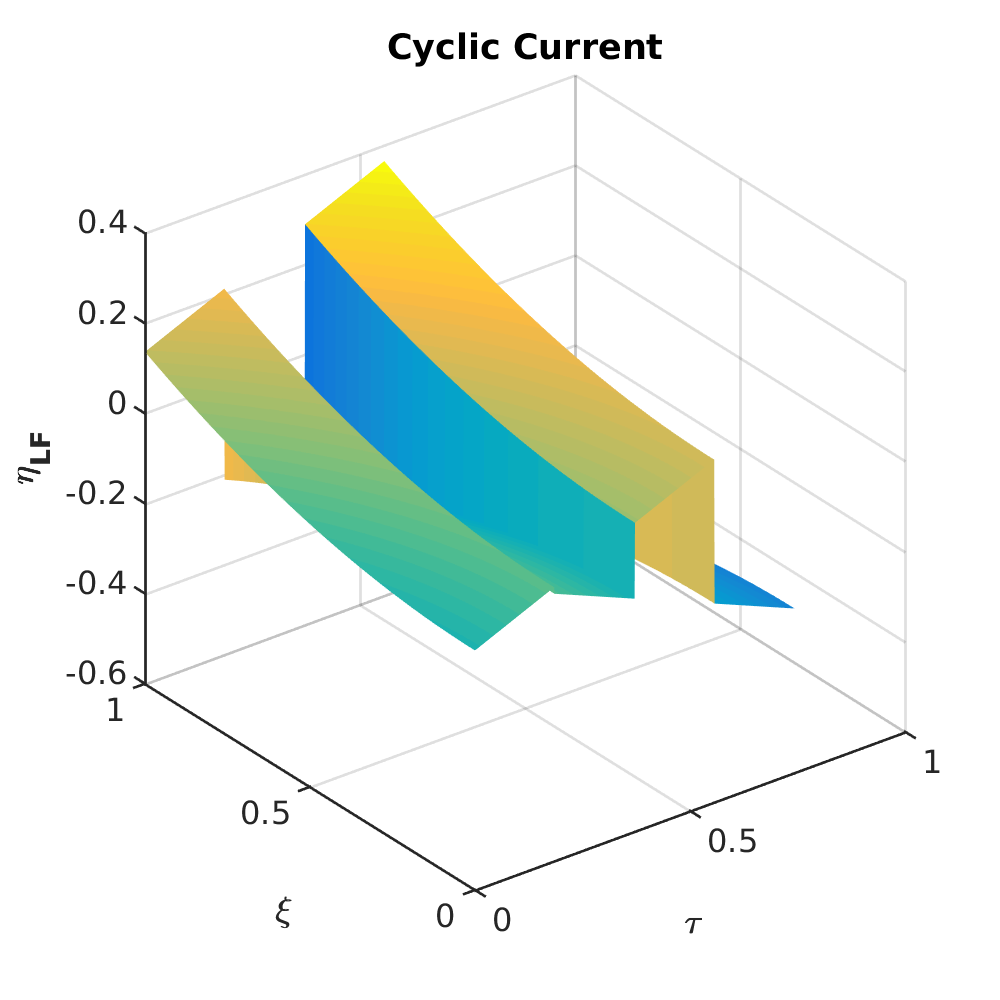
\includegraphics[trim = 0in 0in 0in 0in, clip, width=0.7\textwidth]{figures/etaLF3d_cycl.png}      
    \caption{Solution of LF model for cyclic current.}
    \label{fig:etaLF_cycl}
\end{figure}
%%

%%
\begin{figure}[h]
    \centering
    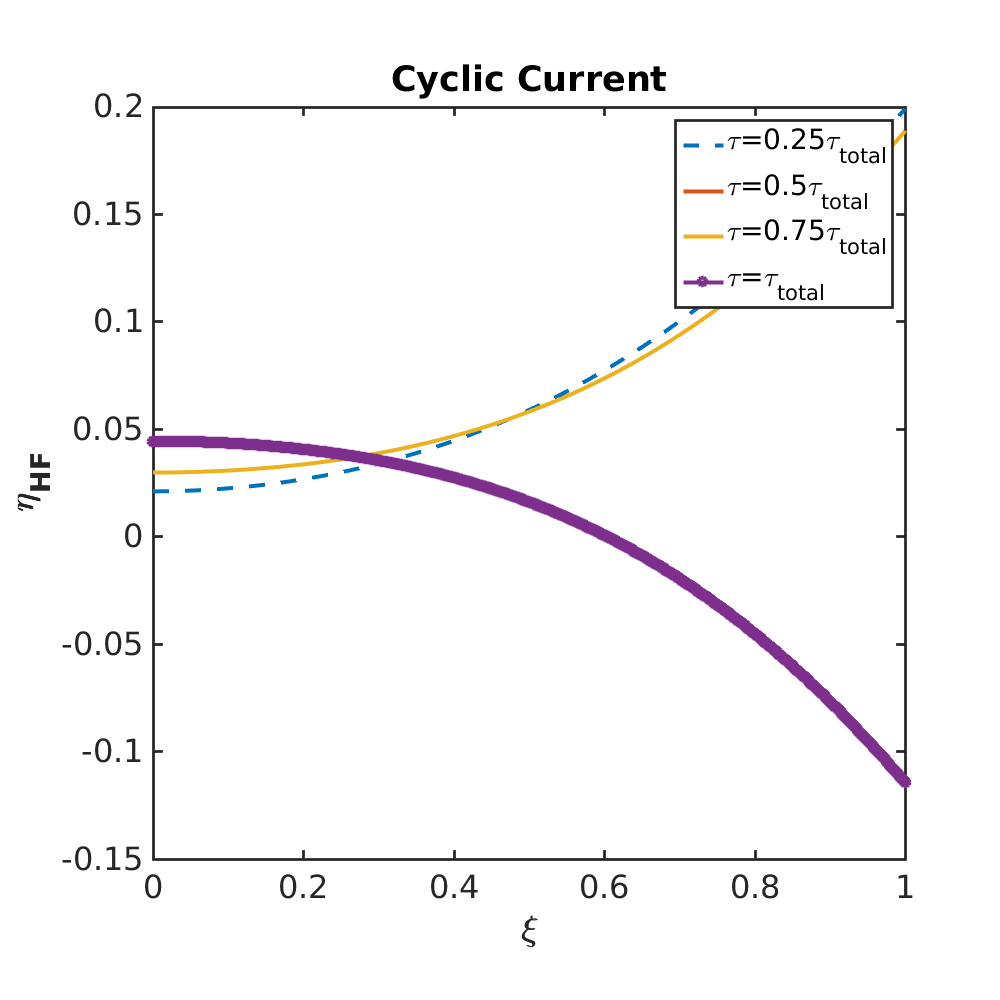
\includegraphics[trim = 0in 0in 0in 0in, clip, width=0.7\textwidth]{figures/etaHF2d_cycl.png}
    \\
    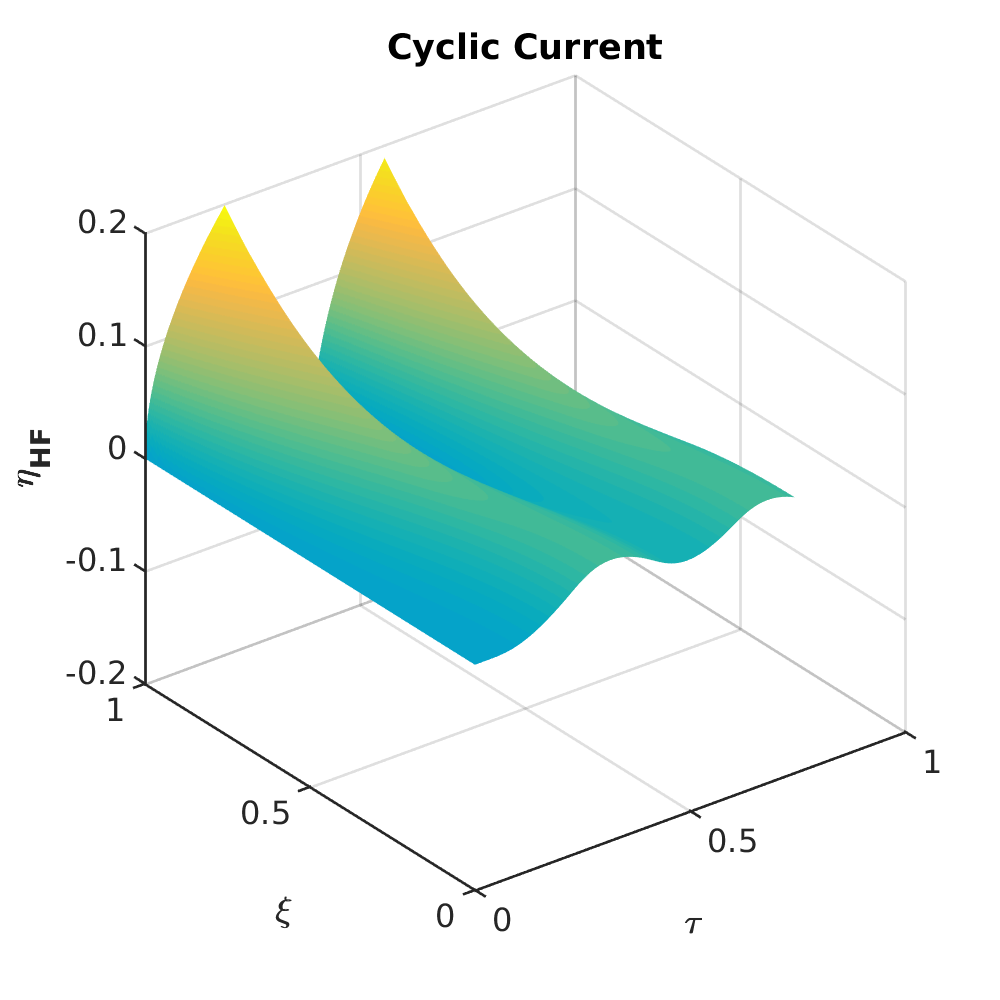
\includegraphics[trim = 0in 0in 0in 0in, clip, width=0.7\textwidth]{figures/etaHF3d_cycl.png}      
    \caption{Solution of HF model for cyclic current.}
    \label{fig:etaHF_cycl}
\end{figure}
%%

%%
\begin{figure}[h]
    \centering
    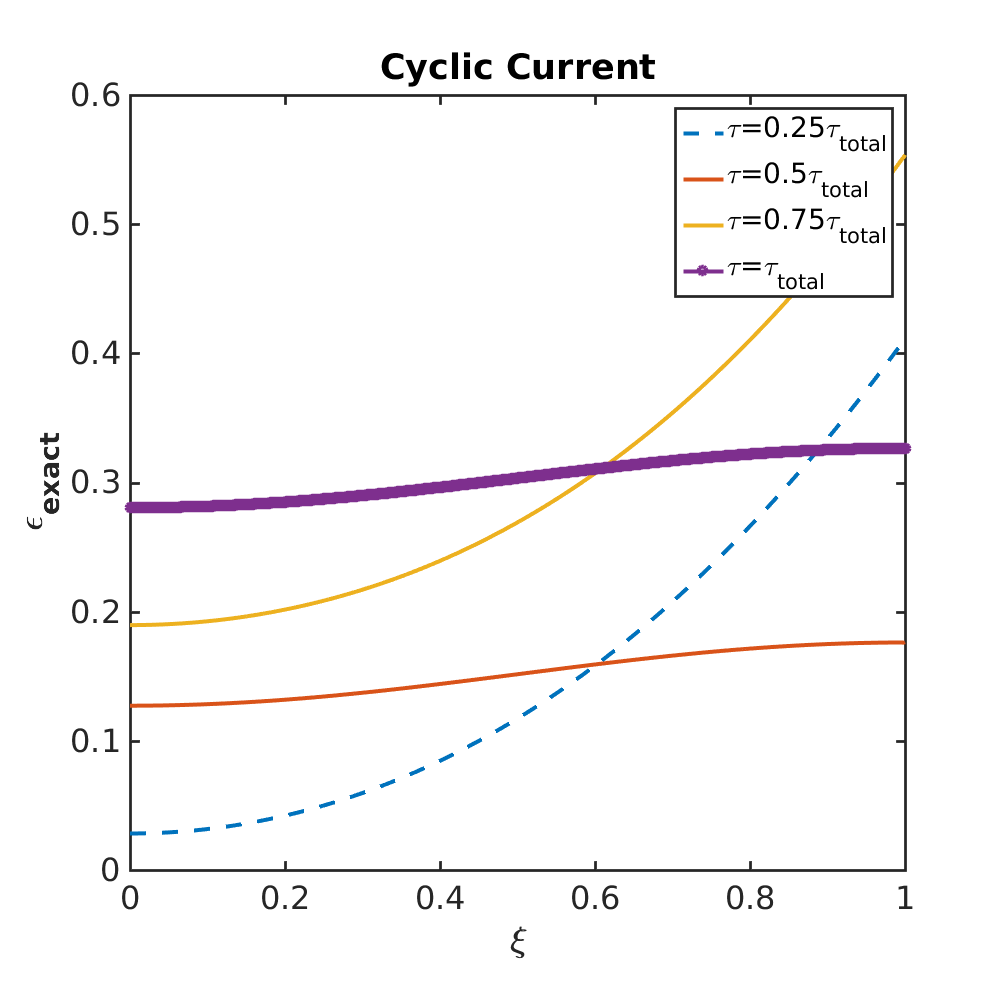
\includegraphics[trim = 0in 0in 0in 0in, clip, width=0.7\textwidth]{figures/error2d_exact_cycl.png}
    \\
    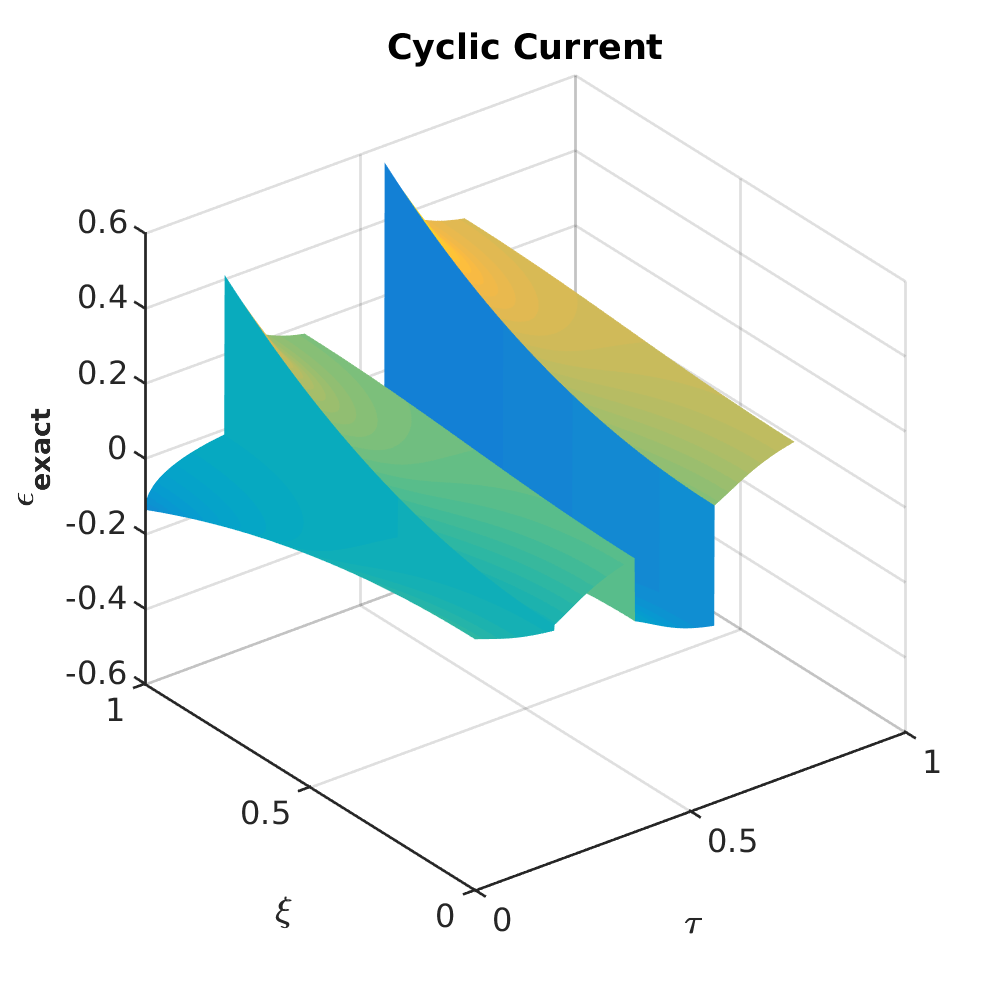
\includegraphics[trim = 0in 0in 0in 0in, clip, width=0.7\textwidth]{figures/error3d_exact_cycl.png}       
    \caption{Solution of error $\epsilon(\xi,\tau)$ at different normalized time and space.}
    \label{fig:error_2d_cycl}
\end{figure}
%%


%%
\begin{figure}[h]
    \centering
    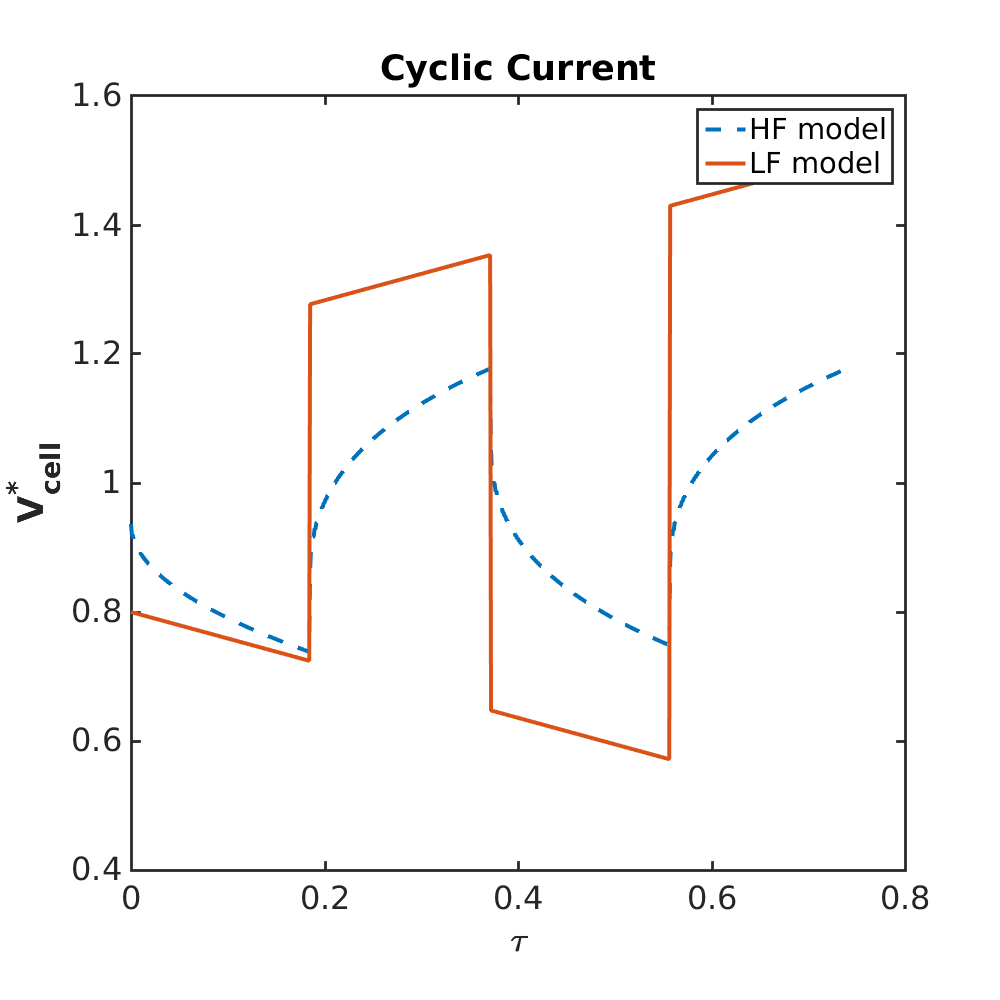
\includegraphics[trim = 0in 0in 0in 0in, clip, width=1.1\textwidth]{figures/Vcell_cycl.png}      
    \caption{Change in voltage across the porous electrode with dimensionless time for cyclic current.}
    \label{fig:Vcell_cycl}
\end{figure}
%%


%========================================================================
% Bibliography
%========================================================================
\clearpage
%\nocite{*}       
\bibliographystyle{abbrv}  % Here the bibliography 		     %
%\bibliography{diss}        % is inserted.			     %
\bibliography{refs}
\index{Bibliography@\emph{Bibliography}}%

\end{document}
